%% LyX 2.0.2 created this file.  For more info, see http://www.lyx.org/.
%% Do not edit unless you really know what you are doing.
\documentclass[english]{article}
\usepackage[T1]{fontenc}
\usepackage[latin9]{inputenc}
\usepackage{float}
\usepackage{graphicx}
\usepackage{babel}
\begin{document}

\title{TSK-Typer Functional Specification - v.1.2}


\author{Saba Saba}

\maketitle
\pagebreak{}

\tableofcontents{}\pagebreak{}

\listoffigures


\pagebreak{}


\section{Overview}

The touch-sensitive keyboard (TSK) is a keyboard that can detect a
user's fingers resting lightly on the keys. TSK-Typer is a typing
game that leverages the TSK's functionality to determine the typist's
posture while using the application.


\paragraph*{Disclaimer: This specification is not complete, and is subject to
revision.}


\section{Non-Goals}

TSK-Typer is not intended to deal with TSK's keyboard gesture functionality. 


\section{Scenarios}

Scenarios are provided below to better understand the cases where
a user would use TSK-Typer.
\begin{enumerate}
\item Robert is a zookeeper with aspirations of becoming a celebrated novelist.
To achieve this goal, he purchases hundreds of computers. He then
forces the zoo's chimpanzees to type for long hours every day. Since
progress is slow, he installs TSK-Typer on each computer. Thus, he
hopes to improve the chimpanzees' typing skills and subsequently gain
a novel in the process.
\item Jim is a competitive video-gamer who wants to enter the big leagues.
However, he finds himself looking down at his keyboard when entering
keyboard commands. Furthermore, it is difficult to make out each letter
with only the dim glow of the monitor illuminating the keyboard. Naturally,
this prevents him from climbing up in the ranks. To gain an edge over
his opponents, he installs TSK-Typer to improve his hand-eye coordination
and typing speed.
\end{enumerate}

\section{Screen Specification}

TSK-Typer features a few different screens that the user interacts
with. Each screen is described below from the user's perspective.


\subsection{Setup Screen}

The setup screen is the initial screen displayed to the user. The
text area contains the text that the user will type in the typing
screen. The user can choose to load the contents of a text file into
the text area. This is accomplished by selecting a file name from
the combo box situated above the text area. The file names listed
in this combo box are retrieved from the \textit{levels} folder in
the TSK-Typer application directory. The folder from which these files
are retrieved can also be changed by checking the \textbf{Show Folder
Selection} check box, which displays a text box and a \textbf{Browse}
button. The text box displays the folder from which the file names
are displayed. A \textbf{Browse} button beside the text box allows
the user to bring up an open folder dialog. If the text box is empty
or contains an invalid folder path, an error indicator is displayed
next to the text box and the combo box is disabled. Alternatively,
this text area can be edited by the user manually. Once the text area
is non-empty, the \textbf{Begin} button is enabled. Clicking the \textbf{Begin}
button switches TSK-Typer to the typing screen.

\begin{figure}[H]
\begin{centering}
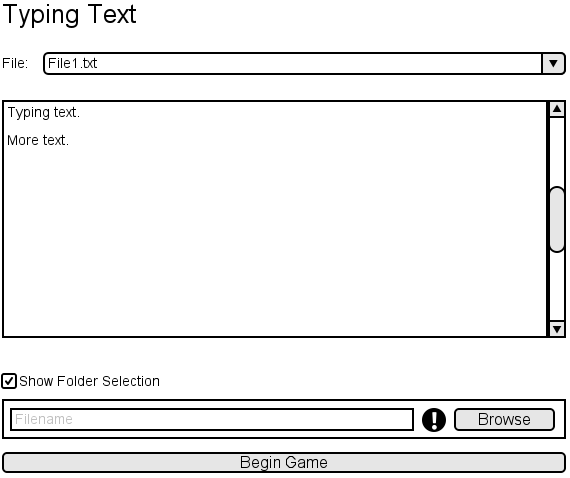
\includegraphics[scale=0.5]{images/setup1}
\par\end{centering}

\caption{Setup screen with folder selection displayed}


\bigskip{}


\begin{centering}
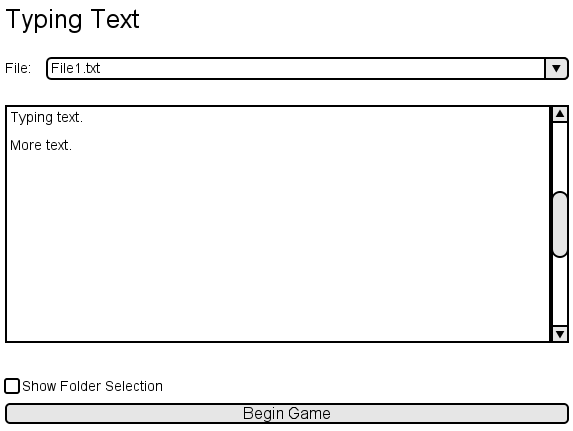
\includegraphics[scale=0.5]{images/setup2}
\par\end{centering}

\caption{Setup screen with folder selection hidden}
\end{figure}



\subsection{Typing Screen}

The typing screen deals with testing the user's typing skills using
text extracted from a given text file. A subset of the text, restricted
to 50 characters, is displayed in a marquee-like display. Each character,
inluding whitespace, is displayed in monospace font. A caret placed
underneath a character denotes the character that the user should
type. When the user presses a key, the character changes colour: green
signifies success, red signifies an incorrect character, and yellow
signifies a correct character typed with incorrect finger placement
on the TSK. Additionally, the text shifts one space to the left whilst
the caret remains in the same position. To make whitespace characters
easier to see, the following representation is used: a single space
is represented as a blank character, a tab is represented by the word
\textbf{Tab} in a box, and a newline is represented by the word \textbf{Return}
in a box. Once every character in the text has been typed, TSK-Typer
switches to the results screen.

\begin{figure}[H]
\begin{centering}
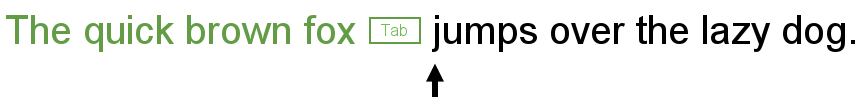
\includegraphics[scale=0.5]{images/typing}
\par\end{centering}

\caption{Typing screen}


\end{figure}



\subsection{Results Screen}

The results screen displays the user's performance statistics. These
statistics are displayed in a table. Additionally, a line chart visible
below the table lists the number of mistakes made by the user over
time. The line chart features two sets of plots: the number of incorrect
characters over time, and the number of characters typed with incorrect
form over time. An overall score is also displayed above the table.
The formula for determining the score is given in figure 5. Note that
a word is considered to be correct if and only if each character is
typed correctly with proper form. A word is considered incorrect if
at least one of the characters typed is incorrect. Finally, a word
is considered to be typed with incorrect form if at least one of the
characters has been typed with incorrect form. This screen features
two buttons: the \textbf{retry} button and the \textbf{settings} button.
Clicking on the \textbf{retry} button results in the TSK-Typer switching
to the typing screen with the same text file loaded. Clicking on the
\textbf{settings} button results in the TSK-Typer switching to the
setup screen.

\begin{figure}[H]
\begin{centering}
Score: 1420
\par\end{centering}

\smallskip{}


\begin{centering}
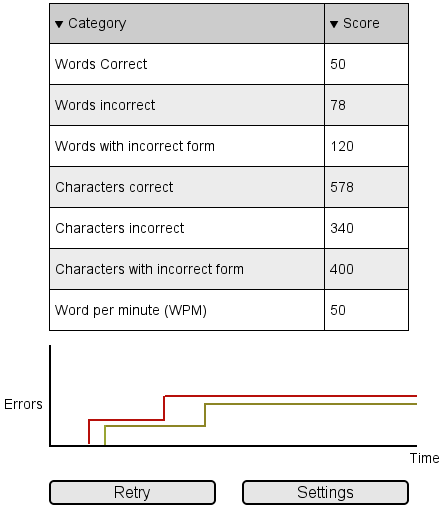
\includegraphics[scale=0.5]{images/results}
\par\end{centering}

\caption{Results screen}
\end{figure}


\begin{figure}[H]
Let $\sigma$ represent the overall score of the user, $s$ is the
words per minute, $w_{g}$ is the number of words typed correctly,
$c_{b}$ is the number of characters typed incorrectly, and $c_{f}$
is the number of characters typed with incorrect form. Hence, the
algorithm for calculating the overall score is:

\[
\sigma=sw_{g}-\left(2c_{b}+c_{f}\right)
\]


\caption{Score algorithm}


\end{figure}

\end{document}
